\section{Prototype Constraints}\label{sec:PrototypeConstraints}
Before the prototype can be established, some considerations have to be made in respect to the time limitations and the main scope of this semester. The aim of the project is to create a functional automated proof of concept lawn mower. The following section includes a brief description of the technology on which the prototype is constructed, along with argumentation for eliminated functionalities.

\subsection{Technology Base}
The technology which has been provided for the prototype is a tracked vehicle, seen on \figref{TrackedVehicle}. The vehicle comes with a brushed DC motor which provides power for rotation of the wheels connected to the belts. Furthermore a servo motor is used to control the ratio of the differential steering, by using breaks connected to the wheels. The tracked vehicle includes two hall sensors, one by each belt, which keeps track of the speed, of the belts, by measuring pulses from magnets mounted on the front wheels. The testing will take place in Aalborg University Vicon Room, where the GoT system is installed and calibrated with the appurtenant transmitter, which is mounted on the tracked vehicle during test.

\begin{figure}[H]
	\centering
	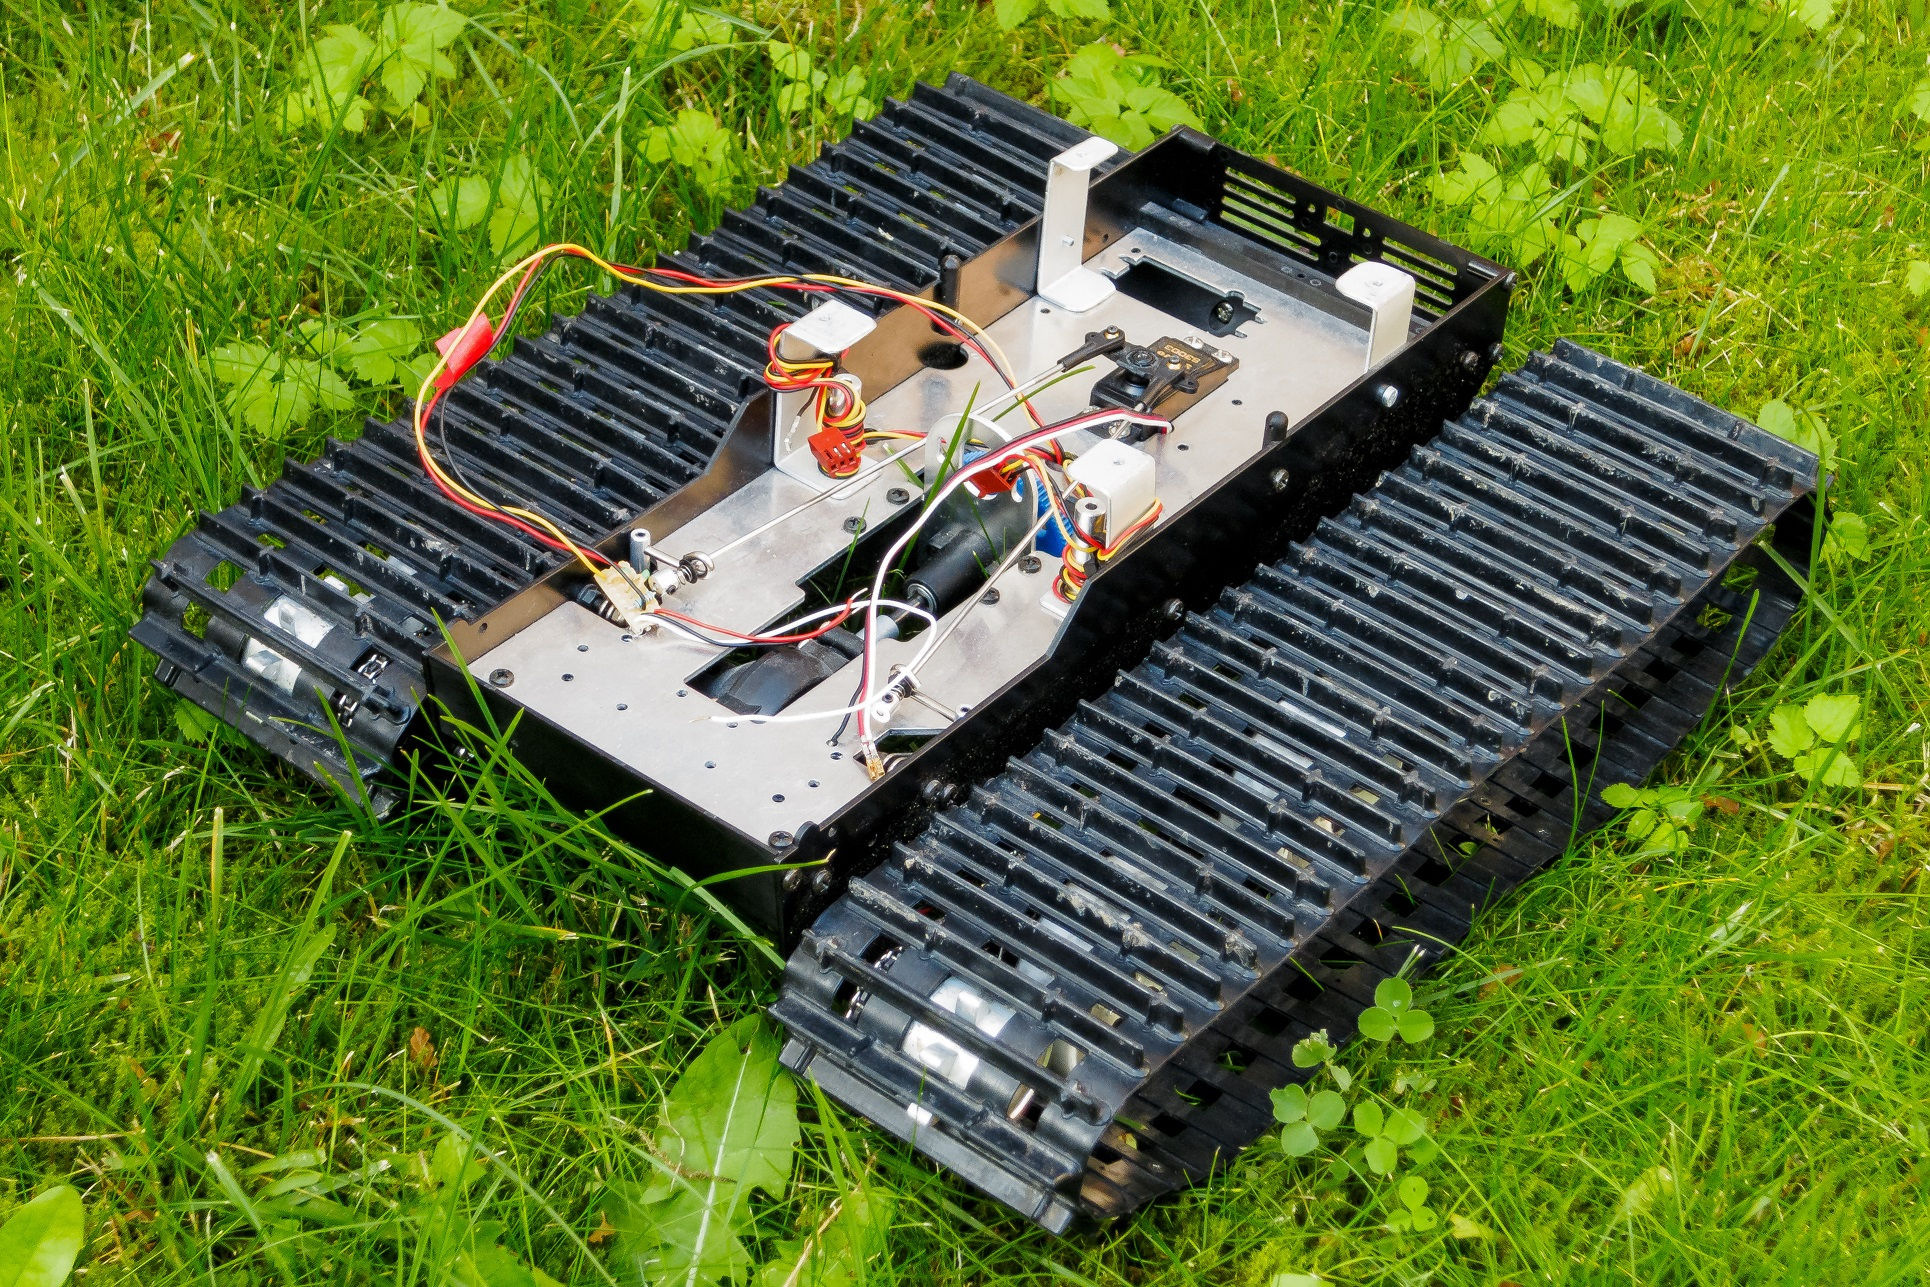
\includegraphics[scale=0.8]{figures/BeltVehicle.jpg}
	\caption{The provided track vehicle}
	\label{TrackedVehicle}
\end{figure}

\todo{datasheet of the vehicle}

\subsection{Grass Length Detection}
Detection of the grass length to control the speed of the lawn mower thus ensuring an evenly cut lawn, is a submodule which can be added at any time. Since it is not fatal for a working system and might even be unnecessary depending on time between each mowing of the lawn, it is decided to exclude this functionality from the initial design.

\subsection{Humidity Sensor}
As the lawn mower is supposed to work outside, it is important to consider that the grass could be humid. Since it is difficult to cut humid grass, a humidity sensor could be used to warn the system of the humidity. Thus the system could go back to the charging station. This submodule is not fatal for the system to be working, so this type of sensor will not be necessary in a prototype design.

\subsection{Obstacle Avoidance}
The lawn movers path might not always be clear, e.g. garden tools, tables or moving objects could be in the way. The vehicle should be aware of what is in front of it at any time, to correct its path and get around the obstacle if necessary. To avoid this the sensor could be a pushing button to detect a solid object or an ultrasound detector if the object is fragile.
As the aim of the project is to control the path of the vehicle by using angular positioning sensors, a proximity sensor will not be included. Static objects could be registered on the map to avoid these issues.\\\\
Furthermore the edge mapping functionality will not be included in the project which instead will focus on a quadratic map predefined in the test room.

\subsection{Power Monitoring}
Power monitoring could be implemented by measuring the voltage across the batteries, to ensure that the lawn mower is not running out of power, and to ensure the vehicles calculated route passes the charging station before the power runs too low.
This and the charging station will not be in the prototype, since it is beyond the scope of the project this semester and is not crucial for a working prototype.

\subsection{Blade Control \& Blade Monitor}
To get the blade to cut the grass evenly over the whole lawn, the blade control and monitor is needed to keep the blade at the same speed.
The blade, and therefore the blade control and monitor, will not be in the prototype. This is because, the focus of the project is on the movement of the vehicle and the blade does not contribute to this and is therefore not needed.
